\chapter{Differential Geometry}
As we have noted before, general relativity is a inherent local theory. It is
convenient to formulate it in terms of differential geometry.
\section{Manifolds}
\begin{definition}
A $n$ dimensional manifold $M$ is a Hausdorff space with countable basis, that
is locally homeomorphic to $\mathbb{R}^n$. We will give a short introduction to
the most important terms.
\end{definition}
%TODO picture
\begin{remark}
The requirements Hausdorff and countable basis are of a more technical nature and are satisfied for most of the objects one can imagine 
except some pathological examples (we won't go into the details on this).

Locally homeomorphic to $\mathbb{R}^n$ means there exists a set of \emph{charts} 
$(\varphi,U^\varphi)$ called an \emph{atlas} $\mathcal{A}$ with $\cup_{\varphi\in\mathcal{A}} U^\varphi =M$, 
i.e. the charts cover the whole manifold. The maps $\varphi:U^\varphi\to \varphi(U^\varphi)\subset\mathbb{R}^n $ are homoemorphisms, 
meaning that $U^\varphi$ is open, $\varphi$ is bijective and both $\varphi$ and $\varphi^{-1}$ are continuous.
Further for any two $\varphi,\psi\in \mathcal{A}$, the coordinate changes 
$\varphi\circ\psi^{-1}:\psi(U^\psi\cup U^\varphi)\to \phi(U^\psi\cup U^\varphi)$
be smooth\footnotemark .
\end{remark}
\begin{figure}
    \begin{center}
        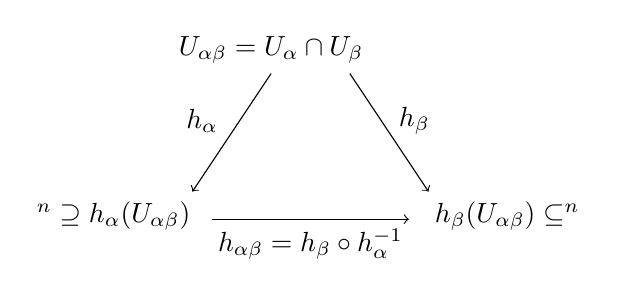
\begin{tikzpicture}
            \draw [->] (1,1.5) -- (0,0);
            \draw [->] (2,1.5) -- (3,0);
            \draw [->] (0.25,-0.35) -- (2.75,-0.35);
            \node [below] at (-1,0) {$\Reals^n \supseteq h_\alpha(U_{\alpha\beta}) $};
            \node [above] at (1,1.5) {$U_{\alpha\beta} = U_\alpha \cap U_\beta$};
            \node [below] at (4,0) {$h_\beta(U_{\alpha\beta}) \subseteq \Reals^n$};
            \node [left] at (0.45,0.9) {$h_\alpha$};
            \node [right] at (2.5,0.9) {$h_\beta$};
            \node [below] at (1.5,-0.35) {$h_{\alpha\beta}= h_\beta \circ h_\alpha^{-1}$};
        \end{tikzpicture}
    \end{center}
    \caption{Coordinate change.} %TODO better caption.
    %TODO mor space.
\end{figure}
\footnotetext{Infinitely often differentiable or short $C^\infty$.}
We can now reduce differentiation on the manifold to the ordinary differentiation in $\mathbb{R}^n$. 
Since physical laws are described in terms of differential equations, we can formulate them on $M$. 
The fact that the coordinate changes are smooth ensures that differentiability
is well defined (and thus the physical laws are).

\begin{sidenote}[Differential Structure]
There can be different \emph{differential structures} on a manifold, 
which means there are multiple (maximal)alases, which
could not be merged because the coordinate changes would not be $C^\infty$. Those differentiable structures therefore imply different notions of differentiability. 
Remarkably this may even play a role in some physical theories. 
As an example an 11d-supergravity can be described as a product
$\Reals^{3+1}\times \Sphere^7$.
Where $\Sphere^7$ is the seven-sphere and $\Reals^{3+1}$ Mikovski space.
This means on every point in the $\mathbb{R}^{3+1}$ there is a (small) $\Sphere^7$  located that contains additional spatial dimensions. 
The $\Sphere^7$ has 28 different differential structures, so the choice of
such a structure affects the theory for the above reasons.
\end{sidenote}
All simple examples we come of can be embedded in a higher space. The
\name{Whitney} embedding theorem states that every real $n$-dimensional Manifold
can be embedded to $\Reals^{2n}$ (This is however not true for complex, i.e. analytic manifolds).
For example the $\Sphere^2$ can be interpreted as submanifold of the $\Reals^3$.
However manifolds are objects that exists independent of such embeddings. 
For example a torus can be thought of as a square with the opposite sides identified (leaving to the left results in re-entering in the left).
\begin{sidenote}[Topology of the Universe]
In addition to the local structure, we may question the global, i.e. the
topological structure of the universe.
On may for example imagine that we live on the surface of a three-sphere (finite
but boundless universe).
However this might be observable in crosscorelation in the cosmic microwave background from photons reaching us 
from different directions but coming from the same event. There is no evidence of such phenomena so far. 
Most models can be excluded to some certainty. A cylindrical
universe is still possible (finite in one, infinite in the
other directions).
\end{sidenote}
\section{Vectors}
Vectors are important objects describing physics. The naive view as an 'arrow
pointing frow one point to another' is flawed.
For example on a sphere an arrow connecting two points does not make much sense.
We want to find a description of vectors as objects that are naturally related to the structure of the manifold independent of the embedding.
\subsection{Definitions}
There are three equivalent definitions for a
(contravariant) vector:
\begin{enumerate}
    \item algebraic 
    \item physical
    \item geometrical.
\end{enumerate}
We start by giving the algebraic definition which is the most
abstract and prefered by mathematicans, because it is suitable for proofs.
Vectors are identified with derivatices, which are formally defined by
\begin{definition}[Derivation]
A derivation $D$ satisfies the following rules, for all $f,g\in
C^\infty(M,\Reals)$ and $\lambda \in \Reals$:
\begin{align}
    D(af+bg) &=Df+Dg\,,\\
    D(\lambda f)&=\lambda f\,,\\
    D(fg)&= (Df)g+f(Dg)\,.
\end{align}
\end{definition}
We then define a vector by 
\begin{definition}[Vector,
algebraic] A vector in $p$ is a derivation on the germ at $p$.
\end{definition}
The germ is the set of all functions $f\in C^\infty(M,\Reals)$, where we
identify all functions that are equal in some neighbourhood of $p$, i.e. vectors are local objects.
Given two vectors we can construct a new one, the \emph{Lie bracket}
\begin{equation}
    [X,Y]f:=X(Yf)-Y(Xf)\, .\label{eq:LieBraket}
\end{equation}
The only property that has to be checked is that it satisfies the Leibniz rule.
\begin{equation}
    XY(fg)=X[(Yf)g+f(Yg)]=(XYf)g+(Yf)(Xg)+(Yg)(Xf)+(XYg)f\\
\end{equation}
Subtracting $YX(fg)$ proves that $[X,Y]$ is indeed a vector. The fact that we
have a natural vectorspace structure on the set of vectors at $p$ motivates the
following
\begin{definition}
The Tangentspace $T_pM$ is the space of all vectors in $p\in M$.
\end{definition}
A basis of $T_pM$ is given by the derivation along the
coordinates $\partial_i$, therefore its dimension is equal to that of the manifold $M$.
Proof sketch:
\begin{enumerate}
    \item Show $f(x^i)=f(0)+x^i\tilde{f}(x^i)$
    \item Write $X=a^i\partial_i$
    \item Show $Xf=0\quad \forall f \iff X=0$
\end{enumerate}
Every vector $A$ can be written as $A=A^i\pd{}{{x^i}}$, where $A^i$ are the
components of the vector. We can now look how the components of the vector
transform under a change of coordinates (the vector itself is invariant!). 
We usually denote the elements of the transformed systems with a bar.
By the chain rule we have
\begin{equation}
    A= a^k\pd{}{{x^k}}= a^k\pd{\overline{x}^i}{{x^k}}\pd{}{{\overline{x}^k}}\, .
\end{equation}
We can also express $A$ directly in the new basis
\begin{equation}
    A= \overline{a}^i\pd{}{{\overline{x}^i}}\, .
\end{equation}
Comparing the coefficients gives the vector transformation law
\begin{equation}
    \overline{a}^i=a^k\pd{\overline{x}^i}{{x^k}}\label{eq:coefftrafo}\, .
\end{equation}
\begin{definition}[Vector,
physical] A vector with components $A^i$ is a object that transforms according
to \ref{eq:coefftrafo} under a change of coordinates.
\end{definition}
Consider a curve on a Manifold $M$, i.e. a
map $\gamma:\mathbb{R}\to M$, with $\gamma(0)=p$, $\dot{\gamma}(0)=X$. Then $D_X f=\od{}{t}(f\circ\gamma)(0)$ is
a derivative, namely the directional derivative along $X$.
Consider the special curves $\gamma_i(t)=\varphi(p+te_i)$, with $\varphi$ a
chart of $M$. Then $D_{\dot{\gamma}_i} f=\partial_if$,  so $D_{\dot{\gamma}_i}$
represents a the directional derivative and we can relate derivatives to the
geometrical tangent space.

Since we have a basis, we can work in (local) coordinates and will do so most of
the time.
\begin{example}[Lie brackets in local coordinates]
Let $A=A^i\partial_i$, $B=B^i\partial_i$ be vectors, then the \name{Lie} bracket
\eqref{eq:LieBraket} in local coordinates is given as
\begin{equation}
    [A,B]^j=A^i\partial_iB^j-B^i\partial_iA^i\, .
\end{equation}
\end{example}
Since the tangent space is a vector space, we can define its dual space
\begin{definition}[Cotangent space] The cotangent space $T_pM^*$ is the set of
linear maps from $T_pM$ to $\mathbb{R}$, i.e.
\begin{equation}
    T_pM^*:=\{L:T_pM\to \mathbb{R}\, |\, L \text{ linear}\}\, .
\end{equation}
\end{definition}
The cotangent space is again a vector space of the same dimension. Its elements
are called \emph{dual} or \emph{covariant} vectors.
We can define a basis on $	T_pM^*$, which we denote by $\dif x^i$ and  which acts on $T_pM$ via
\begin{equation}
    \dif x^i(\partial_j)=\delta^i_j\, . \label{eq:orthdual}
\end{equation}
It can easily deduced by \eqref{eq:orthdual} that the components of a dual vector transform as
\begin{equation}
    \overline{a}_i=\pd{x^k}{{\overline{x}^i}}a_k\, .
\end{equation}
\begin{remark}[Dual vectors in euclidean space]
If $\vec{a},\vec{b}\in\mathbb{R}^n$ contain the components of a vector and a
dual vector respectively, then the transformation can be written in matrix form
\begin{align}
    \vec{a}&\to\overline{\vec{a}}= V\vec{a}\, ,\\
    \vec{b}&\to\overline{\vec{b}}=\left(V\transpose\right)^{-1}\vec{b}\, ,
\end{align}
with $V_{ij}=\dpd{\overline{x}^i}{{x^j}}$ the
Jacobian of the transformation.
In normal calculus we restrict ourself to orthogonal transformations (i.e.
mapping orthonormal bases onto each other) for which
$\left(O\transpose\right)^{-1}=O$.
Which is the reason why we do not bother to distinguish between vectors and dual vectors because they transform identically. 
In special relativity we have e.g.
$\left(\Lambda\transpose\right)^{-1}\neq\Lambda$ for a boost and the difference
becomes even more important in general relativity where the relation can become arbitrarily complicated.
\end{remark}
\section{Tensors}
From vectors $A$ ,$B$ we can construct new objects with multiple indices that posses well defined transformation behaviour. 
For example consider
\begin{equation}
    \overline{T}^{ij}=a^ib^j\, ,
\end{equation}
which transforms as
\begin{equation}
    T^{ij}=\pd{\overline{x}^i}{{x^k}}\pd{\overline{x}^j}{{x^l}}a^kb^l=\pd{\overline{x}^i}{{x^k}}\pd{\overline{x}^j}{{x^l}}T^{kl}\,
   .\label{eq:tensortrafo}
\end{equation}
We call an object that transforms in this way a \emph{tensor}. 
As with vectors, it is possible to define tensors in a coordinate independent
way.
At this point we will make things easier and only consider the physical
definition, i.e. classify tensors by a transformation according to \eqref{eq:tensortrafo}.

A tensor is said to be symmetric in two indices if it stays invariant when exchanging those indices, e.g.
\begin{equation}
    T_{ab}=T_{ba}\, .
\end{equation}
\begin{remark}
We have not yet established a relation between upper and lower indices, i.e. we have no metric. Expressions of the form
\begin{equation}
    \tensor{T}{^a_b}=\tensor{T}{^b_a}
\end{equation}
therefore make no sense.
\end{remark}
\section{The Metric}
%TODO sort sections
So far we have not defined a length scale on manifolds yet. We will do so now by
introducing a \emph{metric} 
\begin{definition}[Metric]
A metric $g$ on a manifold $M$, is a non-degenerate ($\det(g)\neq 0$), symmetric
covariant two tensor.
\end{definition}
We have already seen examples of metrics for the flat space, e.g. in spherical coordinates $g$ was given as
\begin{equation}
    g=
    \begin{bmatrix}
        1 & 0\\
        0 & r^2\\
    \end{bmatrix}\,.
\end{equation}
A metric that is positive definite is called \emph{Riemanian metric}. In
relativity we deal with \emph{Lorentzian metrics}, for which there are vectors
beside the zero vector which have zero 'length'. In flat space we have
$\tensor{g}{_i_j}=\tensor{\eta}{_i_j}$.
\begin{remark}[About
raising and lowering indices] Supose we have given a vector $A=A^i\partial_i$
with coodinates $A^i$, then we can relate it 
in a natural way to a linear form $g(A,\cdot)$,
\begin{equation}
\begin{split}
 g(A,\cdot)\,\colon T_pM &\to \Reals\\
 X &\mapsto g(A,X)\, ,
\end{split}
\end{equation}
i.e. a dual vector. The components of this dual vector are given by its action
on the Basis elemts of the tangentspace
\begin{equation}
A_i=g(A,\partial_i)=A^jg(\partial_j,\partial_i)=g_{ji}A^j\,,
\end{equation}
which is exactly the law for lowering indices. Given the inverse metric we can
multiply this equation by it to obtain $A^i$ in terms of $A_i$.
\end{remark}
\section{Parallel Transport}
Idea: Generalize parralel transport from flat space.
%TODO pictures
If we express a vector in non-cartesian coordinates and shift it it's
coordinates do not change.
We take a look on two operations:
\begin{enumerate}
\item the change of the vector itself
\item the change of its coordinates.
\end{enumerate}
Let $A_i$ be the coordinates of a vector in a system $x^i$ and $B_i$ the in a
system associated with coordinates $y^i$ respectively.
\begin{equation}
A_i=\dpd{{y^j}}{{x^i}}B_j\, ,\quad B_i=d\pd{{x^j}}{{y^i}}A_j\, .
\end{equation}
We look at vectors whose coodinates in the system $y^i$ do not change i.e.
$\delta B_i=0$ The variation of $A_i$ is given by
\begin{equation}
\delta
A_i=\delta\left(\dpd{{y^j}}{{x^i}}\right)B_j
=\md{{y^j}}{2}{{x^i}}{}{{x^k}}{}\delta
x^k B_j\, .
\end{equation}
Expressing $B_i$ in terms of $A_i$ yields
\begin{equation}
\delta A_i = \md{{y^j}}{2}{{x^i}}{}{{x^k}}{}\pd{{x^l}}{{y^j}}A_l\delta x^k
=:\affin{l}{i}{k}A_l\delta x^k
\end{equation}
$\affin{l}{i}{k}$ is called \emph{affine connection} or short affinity.
\begin{remark}
We can always find a coordinate system in wich $\affin{l}{i}{k}\equiv 0$, this
system is called \emph{Riemanian normal coordinate system} (RNCS).
\end{remark}
%TODO construction i.e. geodesic coordinates
We notice that if 
\begin{equation}
\left(\dpd{{A_i}}{{x^j}}-\affin{l}{i}{k}A_l\right)\delta x^k = 0\,
,\label{eq:covdev}
\end{equation}
The vector $A$ does not change its cordinates. We define a \emph{covariant
derivative} 
\begin{equation}
\tensor{A}{_i_;_j}:=\tensor{\nabla}{_j}\tensor{A}{_i}:=\pd{{A_i}}{{x^j}}-\affin{l}{i}{k}A_l\,
.
\end{equation}
It can easyly be seen that the covariant derivative of a tensor transforms as a
tensor, by inspecting \eqref{eq:covdev} and applying the quotient theorem.
\begin{remark}[The
Covariant Derivative in Electrodynamics] Example from Electrodynamics concerning the covariant derivative. 
The theory is invariant under transformations $\phi\to e^{\imI \alpha}\phi$, 
because $\phi^*\phi$ and $\phi^*\nabla\phi-\phi\nabla\phi^*$ do not change.
In order to make the lagrangian gauge invariant we exchange
\begin{equation}
\tensor{\partial}{_\mu}\to\tensor{D}{_\mu}+\imI\tensor{A}{_\mu}\, ,
\end{equation}
%TODO what is phi?
which effectively produces aditional terms in the lagrangian, namely
\begin{equation}
\imI\tensor{A}{^\mu}\left(\phi^*\tensor{\partial}{_\mu}\phi
-\phi\tensor{\partial}{_\mu}\phi^*\right)=\imI\tensor{A}{^\mu}\tensor{J}{_\mu}\,,
\quad\tensor{A}{_\mu}\tensor{A}{^\mu}\phi^2\,.
\end{equation}
The commutator between the covariant derivatives calculates to  
\begin{equation}
\left[\tensor{D}{_\mu},\tensor{D}{_\nu}\right]=\imI \tensor{F}{_\mu_\nu}\,.
\end{equation}
So the noncomutativity is associated with the presence of a field. This is
simmillar to GR where it was related with curvature. 
\end{remark}
Since we have now established a relation between vectors and dual vectors, we
can also determine the covariant derivative of a dual vector. Therefore we
consider the scalar $A_iB^i$. Since the covariant derivative satisfies the
Leibniz rule we get
\begin{align}
\tensor{(A_iB^i)}{_{;j}} =
\tensor{A}{_i_;_j}\tensor{B}{^i}+\tensor{A}{_i}\tensor{B}{^i_;_j}
\end{align}
But for scalars the covariant derivative is identical to the normal derivative
so that 
\begin{align}
(A_iB^i)_{;j} =(A_iB^i)_{,j}=
\tensor{A}{_i_,_j}\tensor{B}{^i}+\tensor{A}{_i}\tensor{B}{^i_,_j}
\end{align}
If we put in the covariant derivative of a we get 
\begin{equation}
\tensor{A}{_i}\tensor{B}{^i_;_j}=\tensor{A}{_i}\left(\pd{}{{x^j}}B^i+\Gamma^i_{kj}\tensor{B}{^k}\right)
\end{equation}
Since $A$ was arbitary, we can deduce that
\begin{equation}
\tensor{B}{^i_;_j}=\left(\pd{}{{x^j}}B^i+\Gamma^i_{kj}\tensor{B}{^k}\right)
\end{equation}
for a (1,1)-tensor we get:
\begin{equation}
\tensor{A}{^i_j_;_k}=\pd{}{{x^k}}\tensor{A}{^i_j}-\Gamma^a_{jk}\tensor{A}{^i_a}+\Gamma^i_{ak}\tensor{A}{^a_j}\,
.\end{equation}
Similar expressions hold for tensors of arbitary rank where each index gives an
aditional term containing a contraction with the affinity $\Gamma^i_{jk}$. 
We now want to consider curved spaces. This can not immediatly be determined by
the metric, for example the polar coordinates do not look flat even though they
describe the ordinary $\Reals^2$.
%TODO pictures
\section{Riemanian Curvature Tensor}
%TODO sort section
We can contract indices on the Rieman Tensor
\begin{equation}
\tensor{R}{^i_i_k_l}=\pd{{\Gamma^i_{il}}}{{x^k}}-\pd{{\Gamma^i_{ik}}}{{x^l}}
\end{equation}
which is zero for a metric affinity. The Ricci tensor is given by
\begin{equation}
\tensor{R}{_j_k}=\tensor{R}{^i_j_k_i}\, .
\end{equation}
Because of the symmetrie this are all independent contractions. Notice that at
this point we cannot raise or lower indices to contract different indices.
Since we can express the Rieman tensor in terms of commutators ther is a also a
symmetry that can be derived from the Jacobi identity:
\begin{equation}
\left[A\left[B,C\right]\right]
+\left[C\left[A,B\right]\right]
+\left[B\left[C,A\right]\right]=0\,.
\end{equation}
Physics can be described in terms of differential equations. We for example
would like to have a object similiar to the laplacian in curved coordinates.
However $\partial_i\partial_i$ is not coordinate invariant. We therefore
introduce a metric. The equivalence principle implies that space is locally
Minkovski.
\begin{sidenote}
There are certain theories that can be formulated without a metric. An example
beeing threedimensional gravity, which is nondynamic. 
\end{sidenote}
Inner product 
\begin{equation}
g(A,B)=\tensor{g}{_i_j}\tensor{A}{^i}\tensor{B}{^j}
\end{equation}
Pseudo norm
\begin{equation}
\|A\|^2=g(A,A)=\tensor{g}{_i_j}\tensor{A}{^i}\tensor{A}{^j}
\end{equation}
Since the connection and the metric are not related, we stil don't have a lenght
scale on the manifold
% \begin{equation}
% \tensor{R}{_i_j_k_l}:=\tensor{g}{_i_a}\tensor{R}{^a_j_k_l}
% \end{equation}
% Only useful if $R$ and $g$ are related i.e. metric connection.
% (Bilder)
A curve is a map $\gamma:\Reals\to M$. The parametrisation is arbitary e.g.
\begin{equation}
\begin{split}
\gamma:\, &\Reals\to \Reals^2\\
& t\mapsto
\frac{1}{2} t^2
\begin{bmatrix}
1 \\
1
\end{bmatrix}\, ,
\end{split}
\end{equation}
clearly describes a straight line with $y=x$.
We notice that $\od{\tensor{\gamma}{^i}}{t}$ is parallel to
$\od[2]{\tensor{\gamma}{^i}}{t}$. This gives rise to annother possible
generalisation of a straight line.
In curved coordinates we have 
\begin{equation}
\od[2]{\tensor{x}{^i}}{t}+\affin{i}{j}{k}\od{\tensor{x}{^j}}{t}\od{\tensor{x}{^k}}{t}
=\lambda(t)\od{\tensor{x}{^j}}{t}\,.
\end{equation}
%TODO all steps + reasoning
If we demand that this is equal to the minimazation of the arc length we get a
preffered connection. 
Suppose we have a different parametrisation $s(t)$
\begin{equation}
\od{\tensor{x}{^i}}{t}=\od{\tensor{x}{^i}}{s}\od{s}{t}\,,\quad
\od[2]{\tensor{x}{^i}}{t}=\od[2]{\tensor{x}{^i}}{s}\left(\dod{s}{t}\right)^2
+\od{\tensor{x}{^i}}{s}\dod[2]{s}{t}\, ,
\end{equation} 
then the equation for a straight line reads as
\begin{equation}
\left(\dod[2]{\tensor{x}{^i}}{s}+\affin{i}{j}{k}\dod{\tensor{x}{^j}}{s}\dod{\tensor{x}{^k}}{s}
\right)\left(\dod{s}{t}\right)^2+\dod[2]{s}{t}\dod{\tensor{x}{^i}}{s}
=\lambda(t)\dod{\tensor{x}{^j}}{t}\dod{s}{t}\,.
\end{equation}
To get to the usual form of the geodesic equation we choose $s$ so that
\begin{equation}
\dod[2]{s}{t}=\lambda(t)\dod{s}{t}\label{eq:bedaffpara}
\end{equation}
Which is an ordinary differential equation of type $\ddot{s}=\lambda\dot{s}$
that shoud posses a solution. 
For this special choice of parametrisation we have
\begin{equation}
\dod[2]{\tensor{x}{^i}}{s}+\affin{i}{j}{k}\dod{\tensor{x}{^j}}{s}\od{\tensor{x}{^k}}{s}
=0\,.\label{eq:affingeod}
\end{equation}
We therefore have a preferred set of parameters
called affine parameters that satisfy \eqref{eq:bedaffpara}. The character
of the differential equation implies that the affine parameter is only
defined modulo affine transformations $s\to as+b$. This freedom once more
reflects some kind of gauge invariance.
\begin{remark}
Only the symmetric part of the affinity does contribute to
the geodesic equation \eqref{eq:affingeod}. As long as you are on a geodesic you
can always compare lengths without needing a metric, by the affine parameter.
The 'length' defined this way does not have to concede with the length given by
the metric and is also defined for example for lightlike curves (which cannot
be parametrised by the arc length)
\end{remark}
%TODO at this place there is a repetition of the variation principle. what
% should we do with it?
Notice that \eqref{eq:affingeod} is identical to \eqref{eq:geodeq} if we choose
the affinity to be $\affin{k}{i}{j}=\cSym{k}{i}{j}$. This is called the
\emph{metric} or \emph{Christoffel connection}, and we will
always assume it in the following.
A general metric compatible
connection\footnote{$\tensor{\nabla}{_k}\tensor{g}{_i_j}=0$} satisfies
\begin{equation}
\affin{k}{i}{j}=\cSym{k}{i}{j}+\tensor{T}{^k_i_j}
+\tensor{g}{^i^r}\left(\tensor{T}{^s_j_r}\tensor{g}{_s_i}+\tensor{T}{^s_i_r}\tensor{g}{_s_j}\right)
\end{equation}
with the torsion tensor
\begin{equation}
\tensor{T}{^k_i_j}=\frac{1}{2}\left(\affin{k}{i}{j}-\affin{k}{j}{i}\right)
\end{equation}
So that the Christoffel connection is the only metric compatible symmetric
connection.
\begin{remark}
Non-Christoffel connections play a role, for example when dealing with spinors.
\end{remark}
%TODO connect losose ends
\begin{equation}
\tensor{R}{^i_j_k_l}=-\tensor{R}{^i_j_l_k}\,.
\end{equation}
Bianci identites for the Riemann tensor
\begin{equation}
\tensor{R}{^i_j_k_l_{;m}}+\tensor{R}{^i_j_m_k_{;l}}+\tensor{R}{^i_j_l_m_{;k}}=0
\end{equation}
Proof: If we would write it all out we wold have to write 22 terms. Instead we
use a RNCS so that the Rieman tensor simplifies to 
\begin{equation}
\tensor{R}{^i_j_k_l}
=\tensor{\partial}{_k}\affin{i}{j}{l}
-\tensor{\partial}{_l}\affin{i}{j}{k}
\end{equation}
And with $\tensor{\nabla}{_k}=\tensor{\partial}{_k}$ we get
\begin{equation}
\tensor{R}{^i_j_k_l_{;m}}
=\tensor{\partial}{_m}\tensor{R}{^i_j_k_l}
=\tensor{\partial}{_k}\tensor{\partial}{_m}\affin{i}{j}{l}
-\tensor{\partial}{_l}\tensor{\partial}{_m}\affin{i}{j}{k}\,.
\end{equation}
Plugging in gives the result in the RNCS system, but since the equation is
tensorial, it holds in all systems. Notice the similarity to 
\begin{equation}
\tensor{\partial}{_m}\tensor{F}{_a_b}
=\tensor{\partial}{_b}\tensor{\partial}{_m}\tensor{A}{^a}
-\tensor{\partial}{_a}\tensor{\partial}{_m}\tensor{A}{^b}
\end{equation}
Therefore the Biancci identity is identical to the second set of Maxwells
equations
%TODO reference
If the affinity is symetrical $\affin{k}{i}{j}=\affin{k}{j}{i}$ we further have
the identity
\begin{equation}
\tensor{R}{^i_j_k_l}+\tensor{R}{^i_l_j_k}+\tensor{R}{^i_k_l_j}=0
\end{equation}
For a metric affinity $\affin{k}{i}{j}=\cSym{k}{i}{j}$, we can raise and lower
indices
\begin{equation}
\begin{split}
\tensor{R}{_i_j_k_l}
&=\tensor{g}{_i_a}\tensor{R}{^a_j_k_l}\\
&=\tensor{g}{_i_a}\left(\tensor{\partial}{_k}\affin{i}{j}{l}
-\tensor{\partial}{_l}\affin{i}{j}{k}\right)\\
&=\tensor{g}{_i_a}\left(\tensor{\partial}{_k}\tensor{g}{^a^s}\csym{j}{l}{s}
-\tensor{\partial}{_l}\tensor{g}{^a^s}\csym{j}{k}{s}\right)\\
&=\tensor{\partial}{_k}\csym{j}{l}{i}
-\tensor{\partial}{_l}\csym{j}{k}{i}\\
&=\frac{1}{2}\left(
\dmd{{\tensor{g}{_i_l}}}{2}{\tensor{x}{^j}}{}{\tensor{x}{^k}}{}
+\dmd{{\tensor{g}{_j_k}}}{2}{\tensor{x}{^i}}{}{\tensor{x}{^l}}{}
-\dmd{{\tensor{g}{_i_k}}}{2}{\tensor{x}{^j}}{}{\tensor{x}{^l}}{}
-\dmd{{\tensor{g}{_j_l}}}{2}{\tensor{x}{^i}}{}{\tensor{x}{^j}}{}\right)
\end{split}
\end{equation}
where we used the metric compability in the RNCS
($\tensor{\nabla}{_k}\tensor{g}{_i_j}=\tensor{\partial}{_k}\tensor{g}{_i_j}=0$)
. Imideatly we can exctract symmetries
\begin{align}
\tensor{R}{_i_j_k_l}&=-\tensor{R}{_j_i_k_l}\\
\tensor{R}{_i_j_k_l}&=-\tensor{R}{_i_j_l_k}
\end{align} 
If we further introduce multiindices $A=(i,j)$, $B=(k,l)$ (by antisymmetry
there are six independent components for $A,B$ each)
\begin{equation}
\tensor{R}{_A_B} = \tensor{R}{_B_A}
\end{equation}
So $R$ can be thought as a $6\times 6$ maxtrix.
\begin{table}
    \centering
    \begin{tabulars}{rrr}
      	\toprule
		Dimension&Riemann tensor &Ricci tensor \\
		\midrule
		1&0&0\\
		2&1&1\\
		3&6&6\\
		4&20&10\\
		$n$&$\frac{1}{12}n^2(n^2-1)$&$\frac{1}{2}n(n+1)$\\
		\bottomrule
    \end{tabulars}
    \caption{Number of independent components of Riemann
    and Ricci tensor.\label{tab:Nindcomp}}
\end{table}
Table~\ref{tab:Nindcomp} lists the number of independent components of the
curvature tensor and the Ricci tensor in various dimensions. Therby a
ondimensional space is always flat, a twodimensional is characterised by the
curvature scalar $R$ alone and in three dimensions the Ricci tensor is
sufficient to know the Riemann tensor. Therefore four is the lowest dimension in
which the Rieman tensor contains additional information of the curvature of
space.
Formulas 
\begin{equation}
\mathrm{div} A=\tensor{\partial}{_i}\tensor{A}{^i}=\cSym{i}{i}{k}\tensor{A}{^k}
\end{equation}
\begin{equation}
\tensor{\partial}{_k}g=2g\cSym{i}{i}{k}
\end{equation}
\begin{equation}
\cSym{i}{i}{k}=\frac{1}{\sqrt{g}}\tensor{\partial}{_k}\sqrt{g}
\end{equation}
\begin{equation}
\mathrm{div}
A=\frac{1}{\sqrt{g}}\tensor{\partial}{_k}\left(\sqrt{g}\tensor{A}{^k}\right)
\end{equation}
If further $A$ is derived from a potential
$\tensor{A}{_i}=\tensor{\partial}{_i}V$
\begin{equation}
\square V
=\mathrm{div}A
=\frac{1}{\sqrt{g}}\tensor{\partial}{_k}\left(\sqrt{g}\tensor{g}{^k^i}\tensor{\partial}{_i}V\right)\label{eq:quabla}
\end{equation}
%TODO possible outsource to formula section or the like. There are other
% formulaas as well ..
